\documentclass{lecturenotes}

\renewcommand{\vecka}{6}
\newcommand{\tema}{Vektorer}

\setbeamertemplate{footline}[frame number]
\title[Föreläsningsanteckningar EDA016, 2015]{EDA016 Programmeringsteknik för D}
\subtitle{Läsvecka \vecka: \tema}
\author{Björn Regnell}
\institute{Datavetenskap, LTH}
\date{Lp1-2, HT 2015}
 
\begin{document}

\frame{\titlepage}
\setnextsection{\vecka}
\section[Vecka \vecka: \tema]{\tema}
\frame{\tableofcontents}

%%%%%%%%%%%%%%%%%%%%%%%%%%%%%%%%%%%%%%

\subsection{Att göra denna vecka}
\begin{Slide}{Att göra i Vecka \vecka: Förstå vektorer (eng. Arrays)}
\begin{enumerate}
\item Läs följande kapitel i kursboken: 8 \\  
Begrepp: element, vektor, Array, allokering, indexering
\item Gör övning 6: vektor, registrering
\item Träffas i samarbetsgrupper och hjälp varandra 
\item Gör Lab 5: Gissa Tal \\ Om den är för lätt: bygg ut den, gärna med grafik i SimpleWindow
\end{enumerate}
\end{Slide}

\subsection{Vektorer}
% Ide till övning: medelvärde (heltal i vektor) med tillämpning på bonusuträkning. 
%% Quest: Hur ska vi göra med decimaler? (Reellt beslut i kursen krävs då detta ej är def. i kursprog)


\begin{Slide}{Datastrukturer}\footnotesize
En \href{https://sv.wikipedia.org/wiki/Datastruktur}{datastruktur}:
\begin{itemize}
\item kan innehålla många element,
\item har \emph{ett} namn,
\item och man kan komma åt de enskilda elementen.
\end{itemize}

Man kan organisera elementen på olika sätt, t.ex. som listor, träd eller grafer:
\begin{multicols*}{2}
\includegraphics[width=5cm]{img/lista.pdf}\\
\vspace{5mm}
\includegraphics[width=2.2cm]{img/trad.pdf}
\hspace{5mm}
\includegraphics[width=2.2cm]{img/graf.pdf}

\columnbreak
\pause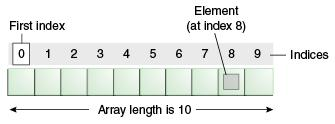
\includegraphics[width=5.5cm]{img/objects-tenElementArray}
\end{multicols*}
\begin{itemize}
\item En \href{}{vektor} \Eng{\href{https://en.wikipedia.org/wiki/Array_data_structure}{array}} är en vanlig datastruktur som är snabb att indexera varsomhelst i.  
\item Kallas även endimensionellt \href{https://sv.wikipedia.org/wiki/F\%C3\%A4lt_\%28datastruktur\%29}{fält} \Eng{one-dimensional array}.
\end{itemize}
\end{Slide} 


\begin{Slide}{Vektorer (arrays) i Java} \footnotesize
Javasyntax för att deklarera \& allokera \href{https://docs.oracle.com/javase/specs/jls/se8/html/jls-10.html} {vektor} \Eng{array} med 10 heltal:
\begin{Code}
int[] nbrs = new int[10];      //typnamn[] = new typnamn[antal];
\end{Code}

\begin{multicols*}{2}
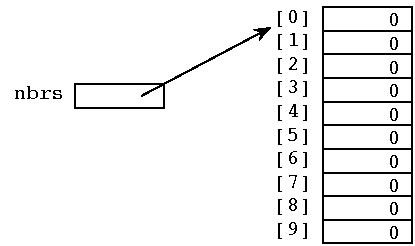
\includegraphics[scale=0.8]{img/vektorbild1.pdf}
\columnbreak
\begin{itemize}\scriptsize
\item Deklarera med hak-parenteser efter typen: \lstinline{int[]}
\item Allokera med \Key{new} och hakar runt antalet platser: \lstinline{new int[10]}
\item Index räknas från \lstinline{0}
\item Indexera med hakparenteser: \\ t.ex. \lstinline{nbrs[3]} ger fjärde platsen
\item Indexering i en tilldelningssats: \lstinline{nbrs[i] = nbrs[i] + 1;} 
\end{itemize}
\end{multicols*}

Fyll vektorn med heltalet 42 på alla platser:
\begin{Code}
for (int i = 0; i < nbrs.length; i++) {  // nbrs.length ger antalet platser 
    nbrs[i] = 42;
}
\end{Code}
\end{Slide} 

\subsubsection{Exempel: Fibonacci}
\begin{Slide}{Vektorer: Exempel Fibonacci}
Fyll vektorn med \href{https://sv.wikipedia.org/wiki/Leonardo_Fibonacci}{Fibonacci}-tal:
\begin{Code}[numberstyle=,numbers=left]
int[] nbrs = new int[10]; 
nbrs[0] = 1;
nbrs[1] = 1;
for (int i = 2; i < nbrs.length; i++) {
    nbrs[i] = nbrs[i - 1] + nbrs[i - 2];
}
\end{Code}
\begin{multicols*}{2}
Efter rad 1:  \\
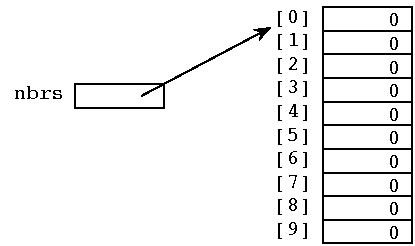
\includegraphics[scale=0.6]{img/vektorbild1.pdf} \\
\columnbreak 
Övning:
\begin{itemize} \scriptsize
\item Rita innehållet i nbrs efter rad 3
\item Rita innehållet i nbrs efter rad 5 för några rundor av \Key{for}-loopen
\item Vad blir innehållet i vektorn efter rad 6? 
\end{itemize}  
\end{multicols*}
\end{Slide} 

\subsubsection{Initialisering av vektorer}
\begin{Slide}{Vektorer: Initialisering och \code{ArrayIndexOutOfBounds}}
\begin{itemize} \footnotesize
\item Vektorer kan initialiseras med ''vektor-initialiserare'' \\ \href{https://docs.oracle.com/javase/specs/jls/se8/html/jls-10.html#jls-10.6}{\Eng{array initializers}} som skrivs med krullparenteser:
\begin{Code}
int[] fibFirstTen = {1, 1, 2, 3, 5, 8, 13, 21, 34, 55};
\end{Code}
\item  Om man indexerar utanför allokerade element med negativt index eller med ett index större än \code{length} kastas ett undantag:
\begin{Code}
System.out.println(fibFirstTen.length);  //skriver ut 10
System.out.println(fibFirstTen[10]); //ArrayIndexOutOfBoundsException
\end{Code}
\item  Observera att det \Alert{inte} ska vara \code{()} efter length.
\item Se även \href{https://docs.oracle.com/javase/tutorial/java/nutsandbolts/arrays.html}{Array tutorial}.
\end{itemize}  
\end{Slide} 

\begin{Slide}{FibonacciArray}
Se exempel \href{https://github.com/bjornregnell/lth-eda016-2015/blob/master/lectures/examples/eclipse-ws/lecture-examples/src/week06/FibonacciArray.java}{\code{week06.FibonacciArray}}:
\lstinputlisting[language=Java, basicstyle=\ttfamily\tiny\selectfont, numberstyle=, numbers=left,]{../examples/eclipse-ws/lecture-examples/src/week06/FibonacciArray.java}
\end{Slide}

\begin{Slide}{FibonacciArrayTest}
\lstinputlisting[language=Java, basicstyle=\ttfamily\scriptsize\selectfont, numberstyle=, numbers=left,]{../examples/eclipse-ws/lecture-examples/src/week06/FibonacciArrayTest.java}
\end{Slide}

\begin{Slide}{Räkna ut medelvärde i Array}
\begin{Code}
public class CollaborationBonus {
    private int[] bonus;
    int nextFreePos = 0;

    public CollaborationBonus(int numberOfGroupMembers){
        bonus = new int[numberOfGroupMembers];
    }
    
    public void addIndividualBonus(int b){
        bonus[nextFreePos] = b;
        nextFreePos++;
    }
    
    public int getGroupBonus(){
        // ÖVNING
     }
}
\end{Code}
\end{Slide}

\subsubsection{Leta efter minimum och maximum i Array}
\begin{Slide}{Leta efter minimum i Array}
\lstinputlisting[language=Java, basicstyle=\ttfamily\tiny\selectfont, numberstyle=, numbers=left,]{../examples/eclipse-ws/lecture-examples/src/week06/MinInArray.java}
\end{Slide}

\begin{Slide}{Leta efter både min och max i ett svep}
\lstinputlisting[language=Java, basicstyle=\ttfamily\tiny\selectfont, numberstyle=, numbers=left,]{../examples/eclipse-ws/lecture-examples/src/week06/MinMaxInArrayBug.java}
\end{Slide}

\subsubsection{Linjärsäkning i Array}
\begin{Slide}{Linjärsökning, pseudokod}
Linjärsökning: \\Börja från början och sök till vi finner; sluta direkt om vi funnit.
\begin{lstlisting}[basicstyle=\ttfamily\fontsize{10}{13}\selectfont]
pos ="platsen för första elementet";
while ( "fler element kvar" && 
        "element på plats pos inte det vi söker"){
    pos = "platsen för nästa element";
}
\end{lstlisting}
\begin{itemize} 
\item Funkar detta även om det inte finns några element?
\item Vad blir  \code{pos} om vi inte hittar något?
\item Vad är \Emph{värsta fallet} för antalet rundor i while-satsen? 
\end{itemize}  
\end{Slide}

\begin{Slide}{Linjärsökning i heltalsvektor}
\lstinputlisting[language=Java, basicstyle=\ttfamily\fontsize{5.8}{6.8}\selectfont, numberstyle=, numbers=left,]{../examples/eclipse-ws/lecture-examples/src/week06/IntFinder.java}
\end{Slide}

\begin{Slide}{Linjärsökning i heltalsvektor, testprogram}
\lstinputlisting[language=Java, basicstyle=\ttfamily\tiny\selectfont, numberstyle=, numbers=left,]{../examples/eclipse-ws/lecture-examples/src/week06/DeepThought.java}
\url{https://www.youtube.com/watch?v=cjEdxO91RWQ}
\end{Slide}

\subsubsection{Vektorer med objektreferenser}
\begin{Slide}{Vektorer med objekt (referensvariabler)}
Javasyntax för att deklarera \& allokera \href{https://docs.oracle.com/javase/specs/jls/se8/html/jls-10.html} {vektor} med 10 objekt:
\begin{Code}
Point[] points = new Point[10];      //Typnamn[] = new Typnamn[antal];
\end{Code}
Array med objektreferenser är \Key{null} från början.
\begin{Code}
Point[] points = new Point[10]; // 10 referenser, alla null från början
// points[0].getX(); // ger NullPointerException
Scanner scan = new Scanner(System.in);
for (int i = 0; i < points.length; i++) {
    int x = scan.nextInt();
    int y = scan.nextInt();
    points[i] = new Point(x, y);
}
\end{Code}
Prova exempel \href{https://github.com/bjornregnell/lth-eda016-2015/blob/master/lectures/examples/eclipse-ws/lecture-examples/src/week06/ArrayWithObjects.java}{ArrayWithObjects}
\end{Slide} 

\begin{Slide}{Programexempel: Polygon}
Klassen \code{PolygonFixedSize} beskriver en polygon med ett givet (maximalt) antal hörnpunkter. Skapa och rita en triangel:

\begin{Code}
PolygonFixedSize triangle = new PolygonFixedSize(3);
triangle.addVertex(10, 10);
triangle.addVertex(50, 10);
triangle.addVertex(30, 40);
triangle.draw(w);
\end{Code}
\end{Slide} 

\begin{Slide}{Implementering av \code{PolygonFixedSize}, del 1}
\begin{Code}
public class Polygon {
    private Point[] vertices; // vektor med hörnpunkter
    private int n;            // antalet hörnpunkter
    
    /** Skapar en polygon som har plats för högst 
        size hörnpunkter */
    public Polygon(int size) {
        vertices = new Point[size];
        n = 0;
    }
    
    /** Definierar en ny punkt med koordinaterna x,y */
    public void addVertex(int x, int y) {
        vertices[n] = new Point(x, y);
        n++;
    }

\end{Code}
\end{Slide} 

\begin{Slide}{Implementering av \code{PolygonFixedSize}, del 2}
\begin{Code}
    /** Flyttar polygonen avståndet dx i x-led, dy i y-led */
    public void move(int dx, int dy) {
        for (int i = 0; i < n; i++) {
            vertices[i].move(dx, dy);
        }
    }
    
    /** Ritar polygonen i fönstret w */
    public void draw(SimpleWindow w) {
        if (n == 0) { return; }
        Point start = vertices[0];
        w.moveTo(start.getX(), start.getY());
        for (int i = 1; i < n; i++) {
            w.lineTo(vertices[i].getX(), 
                     vertices[i].getY());
        }
        w.lineTo(start.getX(), start.getY());
    }
}

\end{Code}
\end{Slide} 

\begin{Slide}{Sätt in element ''mitt i'' vektorn}
\begin{Code}
/** Lägger in en ny punkt med koordinaterna x,y
    Efterföljande element flyttas */
public void insertVertex(int pos, int x, int y) {
    for (int i = n; i > pos; i--) { //flytta "ner" bakifrån
        vertices[i] = vertices[i - 1];
    }
    vertices[pos] = new Point(x, y);
    n++;
}
\end{Code}
\scriptsize Övning: Kör koden med penna och papper. Antag att det finns 2 punkter och rita vektorn vertices efter varje runda i for-loopen.\\
Vad händer om man försöker göra insertVertex \textit{efter} att man har maxantalet punkter?
\end{Slide} 

\begin{Slide}{Ta bort element ''mitt i'' vektorn}
\begin{Code}
/** Tar bort punkten på plats pos. Efterföljande element flyttas */
public void removeVertex(int pos) {
    for (int i = pos; i < n - 1; i++) { //flytta "upp" efterföljande 
        vertices[i] = vertices[i + 1];
    }
    vertices[n - 1] = null;
    n--;
}
\end{Code}
\end{Slide} 

\begin{Slide}{''Utöka'' en vektors storlek}
När vektorn \code{vertices} blir full: 
\begin{enumerate}
\item spara en referens till den gamla vektorn
\item skapa en ny, dubbelt så stor
\item kopiera över elementen från den gamla vektorn till den nya
\end{enumerate}
\begin{Code}
public void addVertex(int x, int y) {
    if (n == vertices.length) {
        Point[] oldVertices = vertices;
        vertices = new Point[2 * vertices.length];
        for (int i = 0; i < oldVertices.length; i++) {
            vertices[i] = oldVertices[i];
        }
    }
    vertices[n] = new Point(x, y);
    n++;
}
\end{Code}
\end{Slide} 

\subsubsection{Registrering}
\begin{Slide}{Algoritmexempel: Registrering}


\begin{Code}
public class Test {
    private Student[] students; // studenterna
    private int n;              // antalet studenter

    /** Skapar ett prov med plats för max studenter */
    public Test(int max) {
        students = new Student[max];
        n = 0;
    }
    
    /** Lägger till studenten s */
    public add(Student s) {
        students[n] = s;
        n++;
    }
    
    /** Skriver ut antalet studenter som har 0,1,...,
        50 poäng på provet */
    public void printStatistics() { ... }
}
\end{Code}
\end{Slide} 

\begin{Slide}{Olika poängintervall}
\lstset{xleftmargin=0mm}

\begin{columns}
\column{2cm}
0, 1, 2, \ldots, 50 poäng:
\column{8cm}
\begin{Code}
public void printStatistics() {
    int[] count = new int[51];
    for (int i = 0; i < n; i++) {
        int index = students[i].getPoints();
        count[index]++;
    }
    // ... skriv ut antalen                       
}
\end{Code}
\end{columns}

\begin{columns}
\column{2cm}
0--9, 10--19,\\ 20--29, 30--39, \\40--50 poäng:
\column{8cm}
\begin{Code}
public void printStatistics() {
    int[] count = new int[5];
    for (int i = 0; i < n; i++) {
        int index = students[i].getPoints() / 10;
        if (index == 5) { // om 50 poäng
            index = 4;
        }
        count[index]++;
    }
    // ... skriv ut antalen  
}
\end{Code}
\end{columns}
\lstset{xleftmargin=\parindent}
\end{Slide} 

\begin{Slide}{Oregelbundna intervall, svårändrad lösning}
0--24 poäng ger betyg U, 25--34 poäng betyg 3, 35--42 poäng betyg 4, 43--50 poäng betyg 5. Antalet U-betyg registreras i \code{count[0]}, antalet 3-betyg i \code{count[1]}, osv.
\begin{Code}
int points = students[i].getPoints();
int index;
if (points < 25) {
    index = 0;
} else if (points < 35) {
    index = 1;
} else if (points < 43) {
    index = 2;
} else {
    index = 3;
}
count[index]++;
\end{Code}
\end{Slide} 

\begin{Slide}{Oregelbundna intervall, \\mer generell \& lättändrad lösning}
\begin{Code}
int[] limits = { 25, 35, 43, 51 };
...
int points = students[i].getPoints();
int index = 0;
while (points >= limits[index]) {
    index++;
}
count[index]++;
\end{Code}
Se hela exemplet här i paketet \href{https://github.com/bjornregnell/lth-eda016-2015/tree/master/lectures/examples/eclipse-ws/lecture-examples/src/week06/register}{week06.register}
\end{Slide} 

\end{document}